\section{Cruscotto delle metriche}
\subsection{Qualità di processo - Fornitura}
\subsubsection{Earned Value, Actual Cost, Planned Value}
\begin{figure}[H]
    \centering
    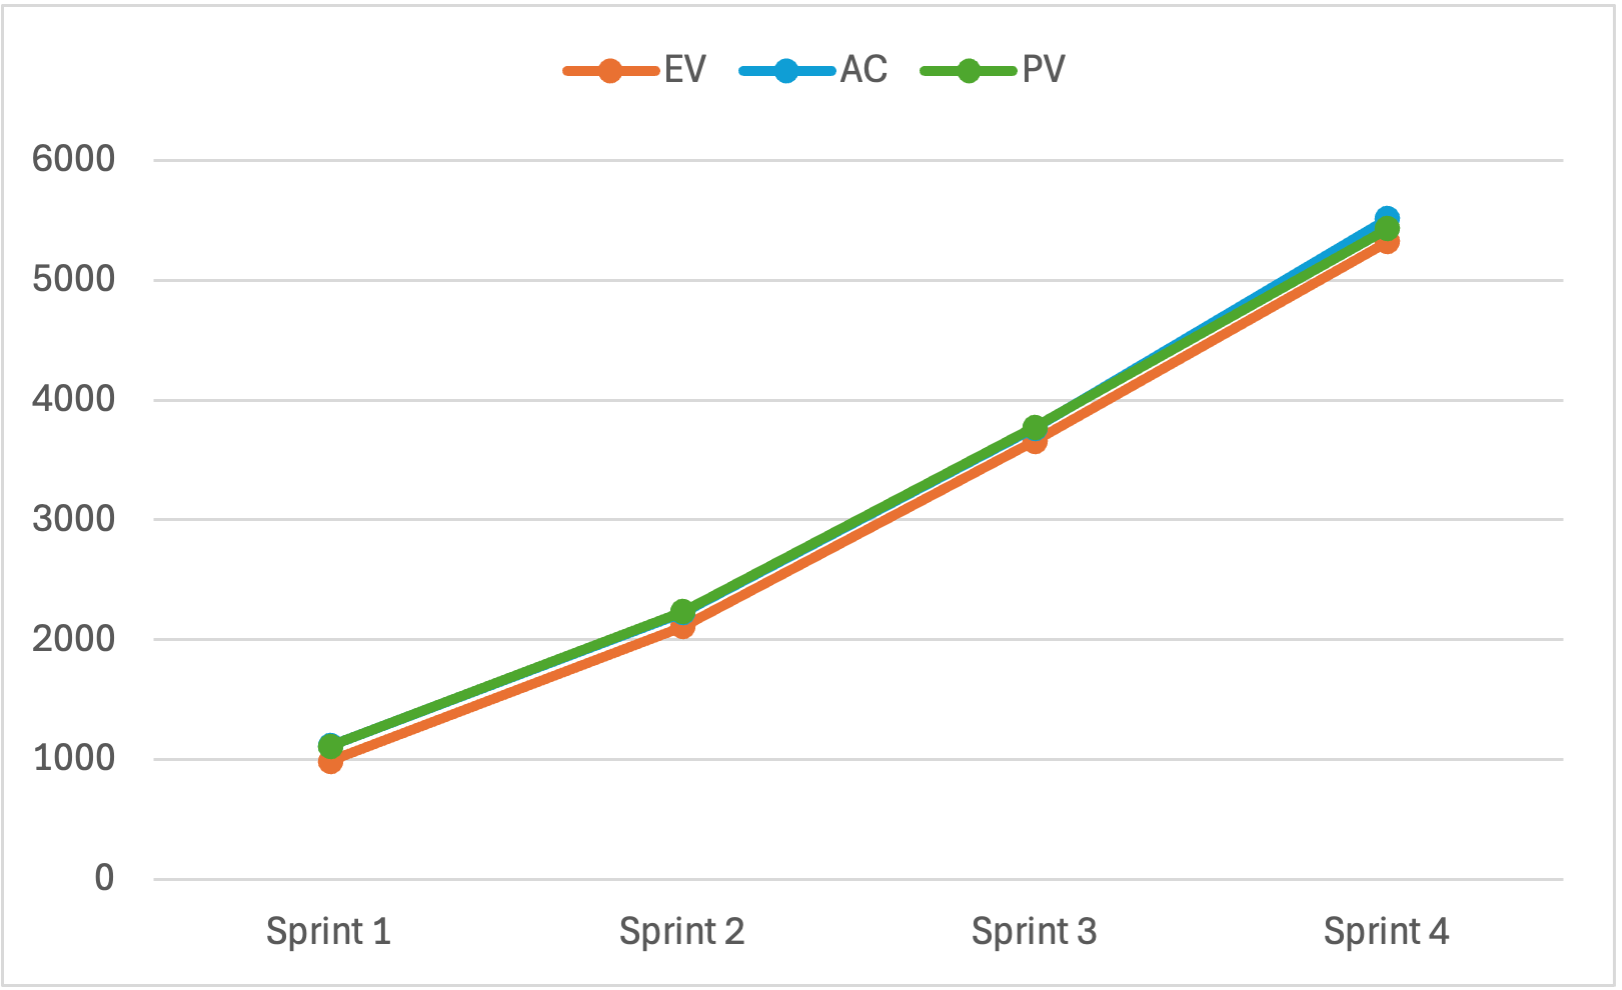
\includegraphics[width=0.8\textwidth]{./images/EV-AC-PV.png}
    \caption{Earned Value, Actual Cost, Planned Value}
\end{figure}
\subsubsubsection*{Analisi}
Queste metriche indicano un buon andamento essendo sempre abbastanza sovrapposte su tutti gli \textit{sprint\textsubscript{G}}, anche se si nota un graduale distaccamento negli ultimi periodi dovuto alle imprecisioni nei costi preventivati.

\subsubsection{Estimated To Completion, Estimated At Completion}
\begin{figure}[H]
    \centering
    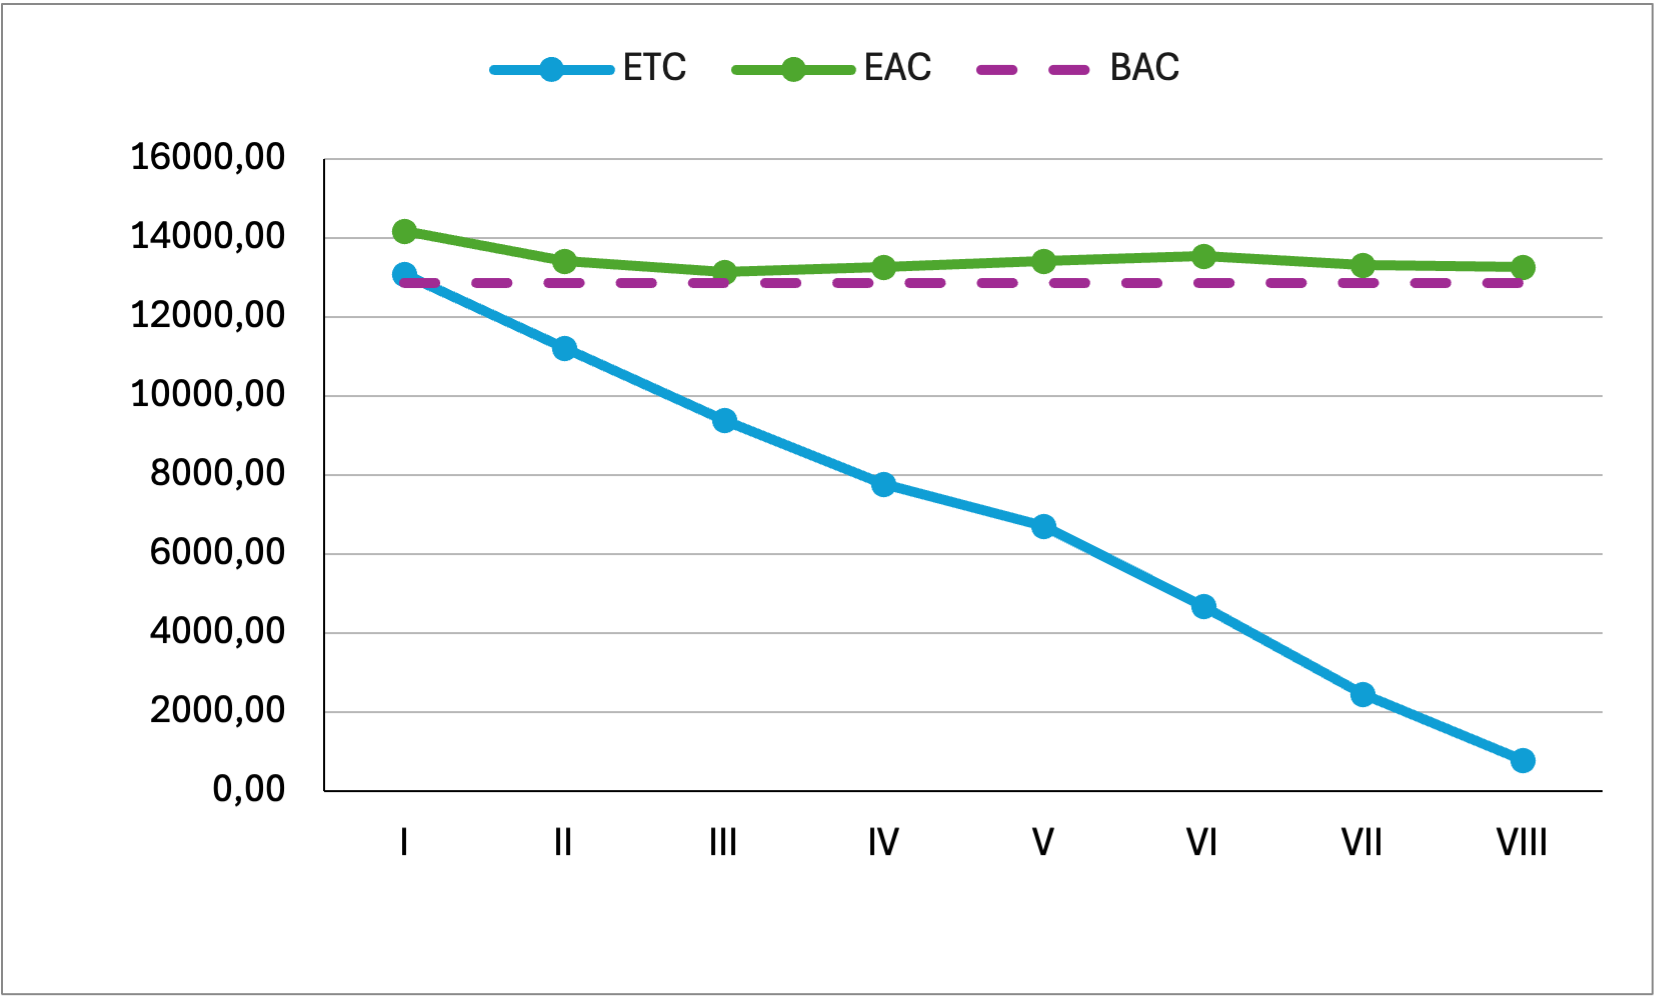
\includegraphics[width=0.8\textwidth]{images/ETC-EAC-BAC.png}
    \caption{Estimated To Completion, Estimated At Completion}
\end{figure}
\subsubsubsection*{Analisi}
Dopo un inizio non ottimale è possibile notare un riallineamento. L'Estimation At Completion si è riallineato al Budget At Completion, ma è sempre rimasto superiore, anche se di poco, a causa del costo maggiore per il raggiungimento di tutti gli obiettivi degli \textit{sprint\textsubscript{G}}. L'Estimated To Completion è sempre stato gradualmente discendente.

\subsubsection{Budget Variance}
\begin{figure}[H]
    \centering
    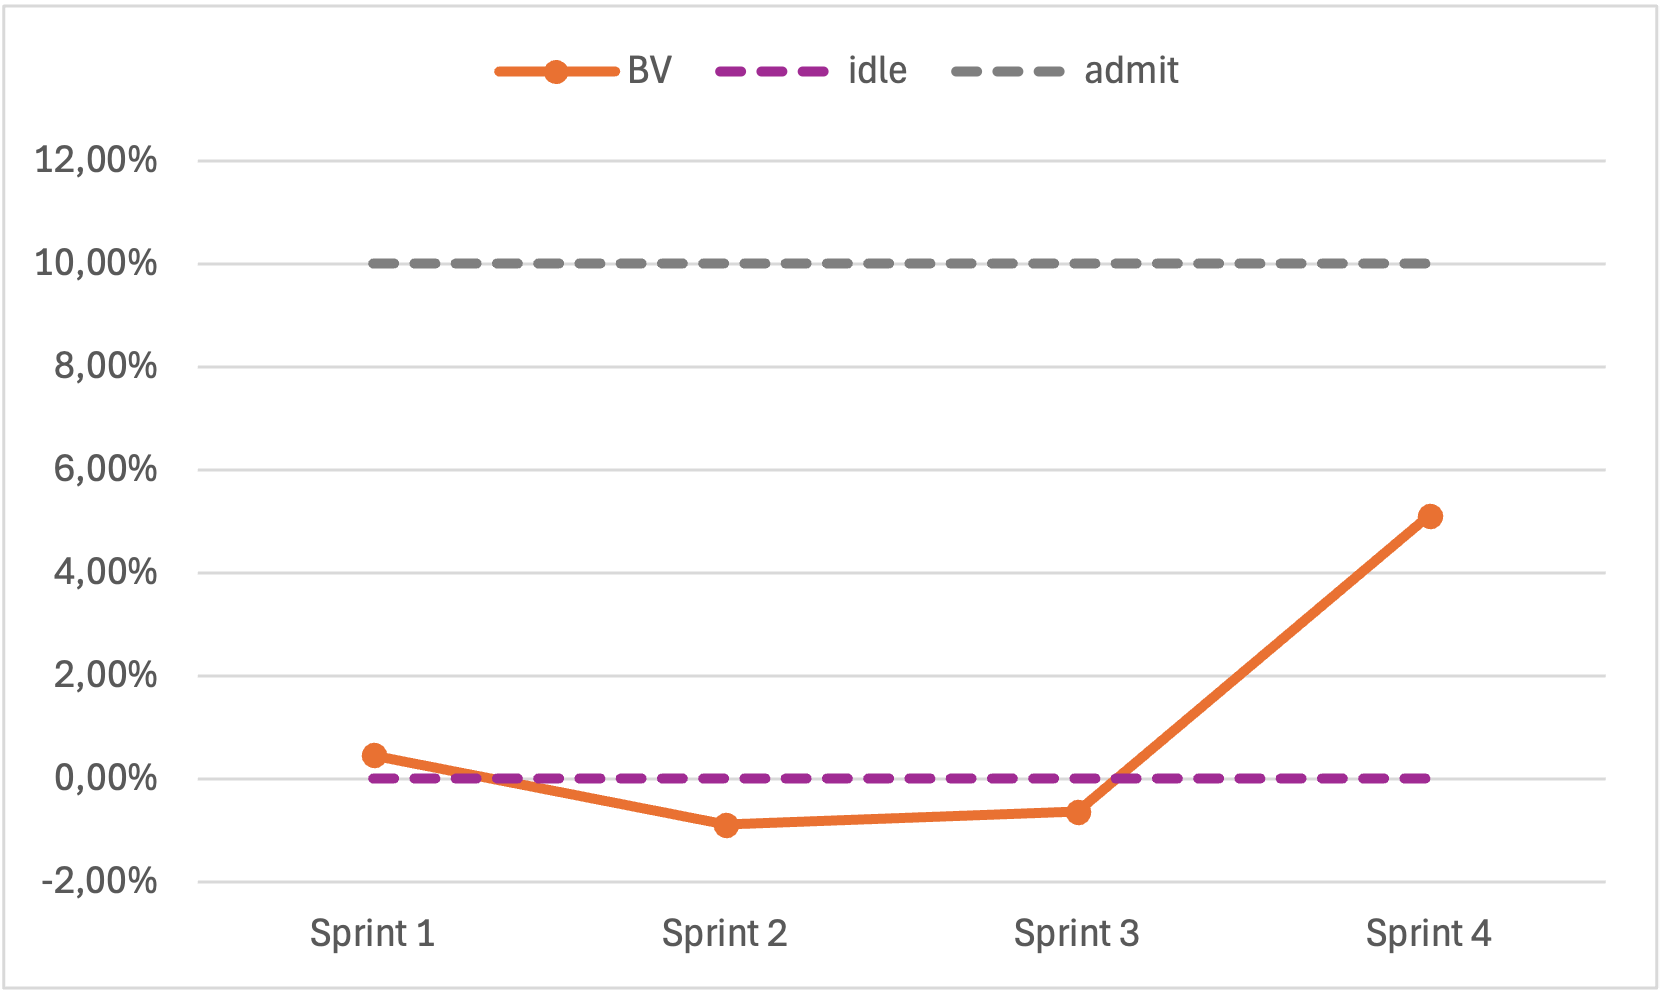
\includegraphics[width=0.8\textwidth]{./images/BV.png}
    \caption{Estimated To Completion, Estimated At Completion}
\end{figure}
\subsubsubsection*{Analisi}
La Budget Variance non sempre è rimasta nei limiti ammissibili come è evidente come nel quarto, quinto e sesto \textit{sprint\textsubscript{G}}. La variazione è stata notevole essendo le ore preventivate  insufficienti e questo è stato un forte segnale di allarme per il gruppo che ha reagito adeguatamente come si può vedere dai due successivi periodo.

\subsubsection{Cost Variance, Schedule Variance}
\begin{figure}[H]
    \centering
    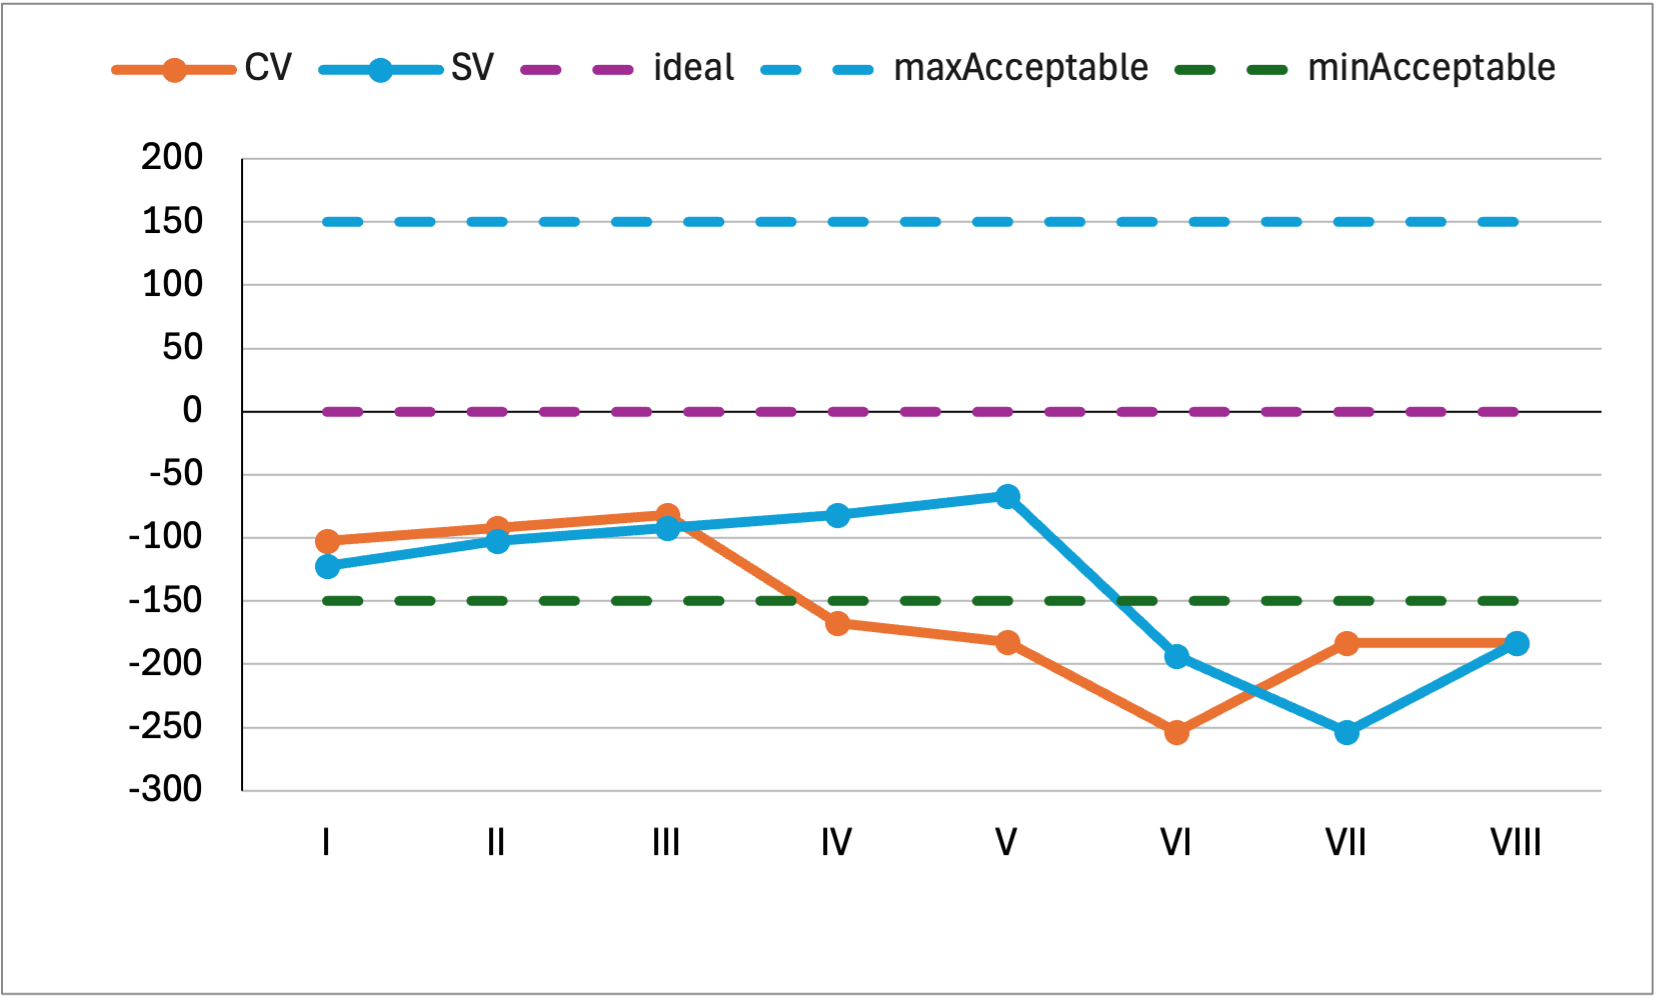
\includegraphics[width=0.8\textwidth]{./images/CV-SV.png}
    \caption{Cost Variance, Schedule Variance}
\end{figure}
\subsubsubsection*{Analisi}
Per quanto i valori non si notano dei netti miglioramenti, ma anzi un peggioramento, a cui il gruppo ha cercato di fare fronte, riuscendoci in parte. Questo indica una not ottimale gestione delle \textit{risorse\textsubscript{G}} per il raggiungimento degli obiettivi entro i costi preventivati.

\subsubsection{Cost Performance Index}
\begin{figure}[H]
    \centering
    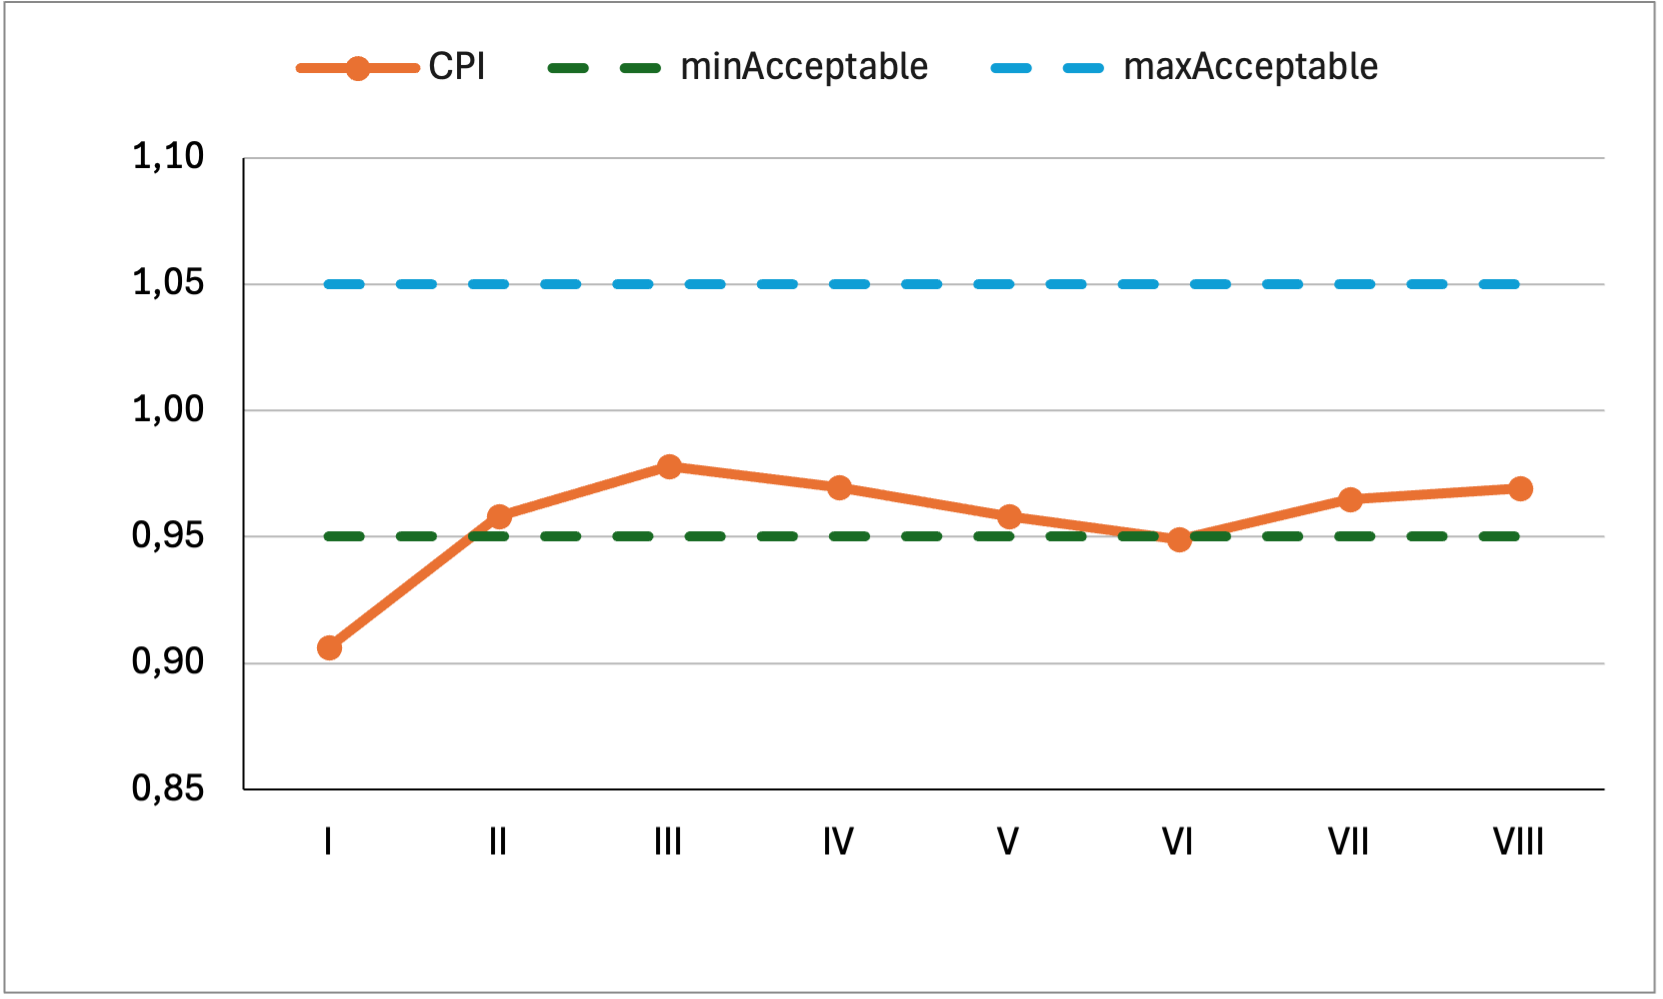
\includegraphics[width=0.8\textwidth]{./images/CPI.png}
    \caption{Cost Performance Index}
\end{figure}
\subsubsubsection*{Analisi}
È evidente come il Cost Performance Index sia migliorato nel corso degli \textit{sprint\textsubscript{G}}, fino a rientrare nei limiti ammissibili e successivamente il gruppo è riuscito a mantenerlo entro tali limiti.

\subsection{Qualità di processo - Documentazione}
\subsubsection{Indice di Gulpease}
\begin{figure}[H]
    \centering
    \includegraphics[width=0.8\textwidth]{./images/GULPEASE.png}
    \caption{Indice di Gulpease}
\end{figure}
\subsubsubsection*{Analisi}
Non solo tutti i documenti rientrano nei limiti accessibili, ma sono anche praticamente tutti in miglioramento nel corso degli ultimi periodi, per quanto il Piano di Progetto che era il documento più carente è rimasto tale. Si nota invece un buon inizio per gli ultimi due documenti creati.

\subsection{Qualità di processo - Gestione della qualità}
\subsubsection{Metriche non soddisfatte}
\begin{figure}[H]
    \centering
    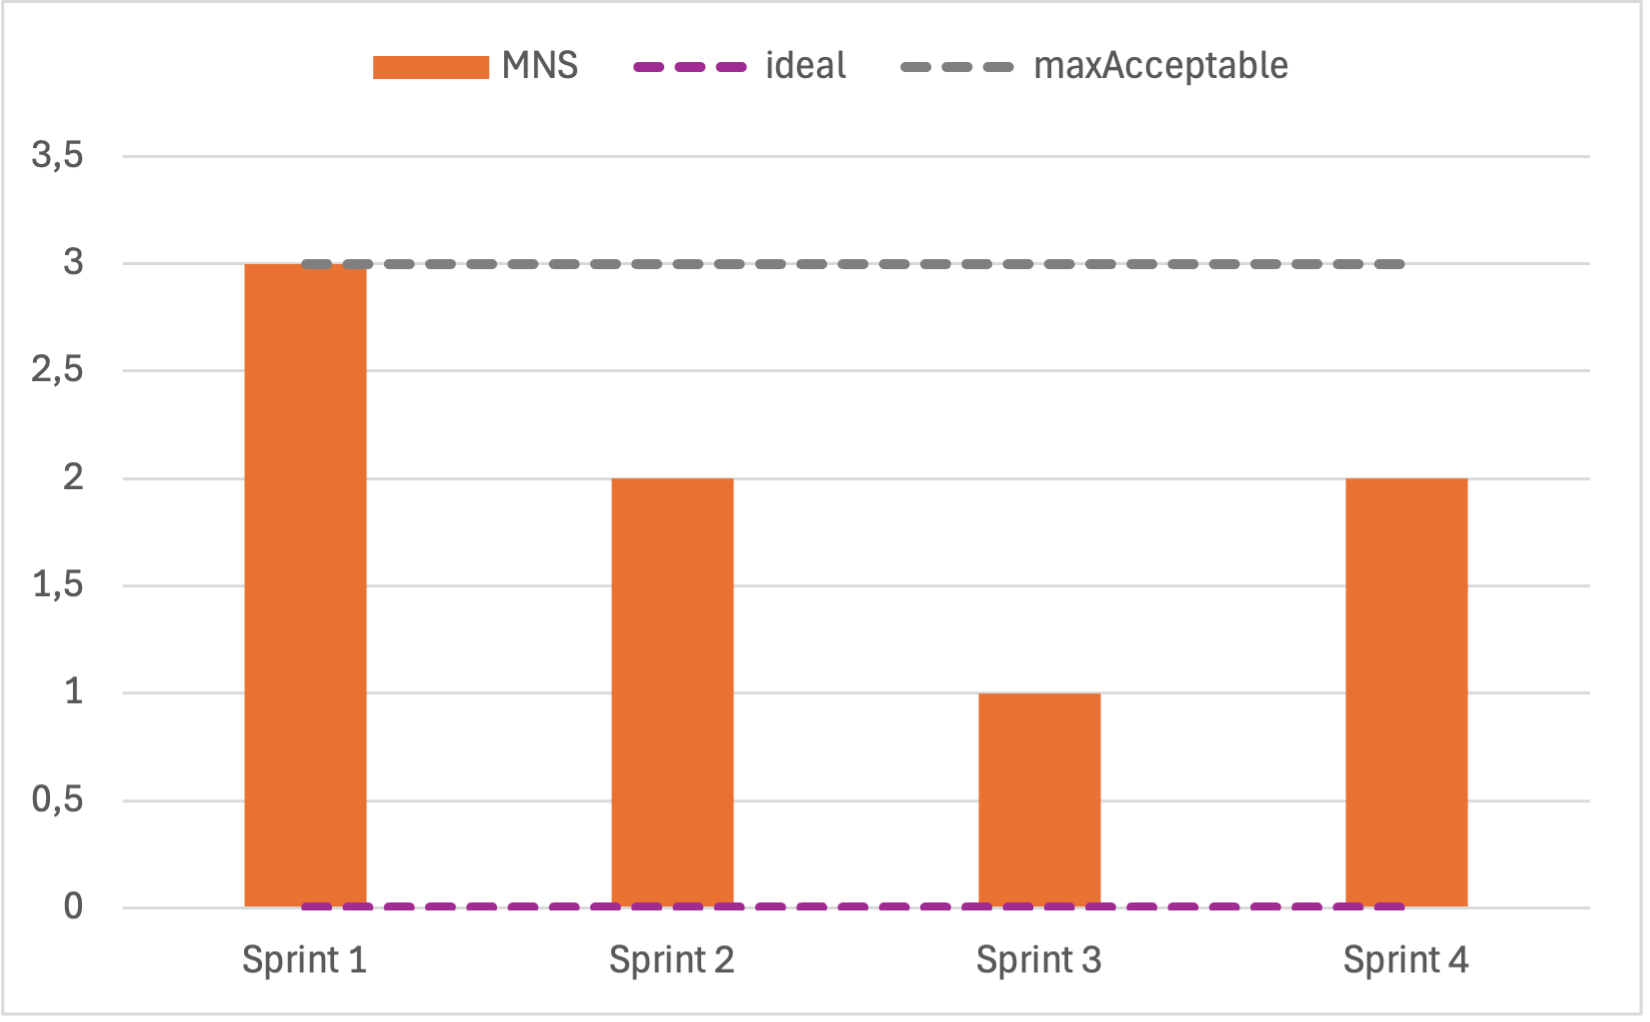
\includegraphics[width=0.8\textwidth]{./images/MNS.png}
    \caption{Metriche non soddisfatte}
\end{figure}
\subsubsubsection*{Analisi}
La metrica che non risulta mai soddisfatta è EAC per la quale si rimanda all'analisi specifica. Altre metriche che risultano non soddisfatte sono ETC (primi due \textit{sprint\textsubscript{G}}), CPI (primo \textit{sprint\textsubscript{G}}) ed infine CV ed SV (dal quinto \textit{sprint\textsubscript{G}} per i quali si rimanda all'analisi specifica).

\subsection{Qualità di processo - Sviluppo}
\subsubsection{Statement Coverage}
\begin{figure}[H]
    \centering
    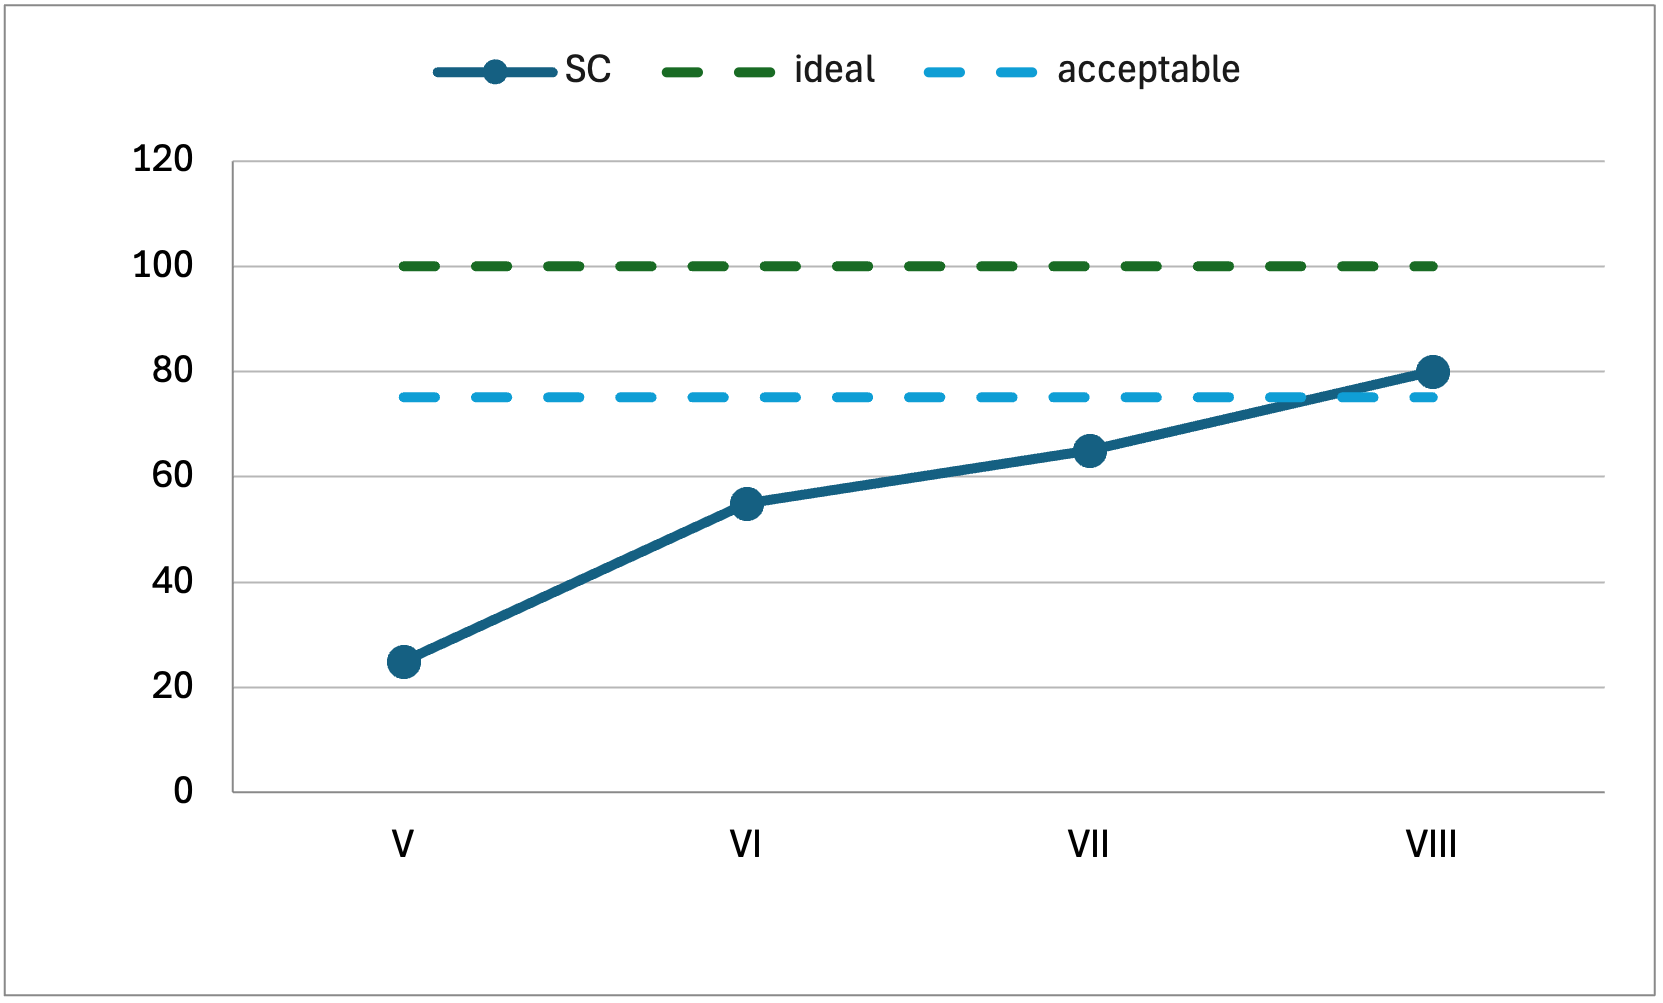
\includegraphics[width=0.8\textwidth]{./images/SC.png}
    \caption{Statement Coverage}
\end{figure}
\subsubsubsection*{Analisi}
 L’incremento della SC indica che non solo vengono testate le funzioni più evidenti, ma si stanno anche affrontando dettagli e scenari più complessi, garantendo che il codice sia eseguito e validato in ogni sua parte.

\subsection{Qualità di prodotto - Funzionalità}
\subsubsection{Requisiti soddisfatti}
\begin{figure}[H]
    \centering
    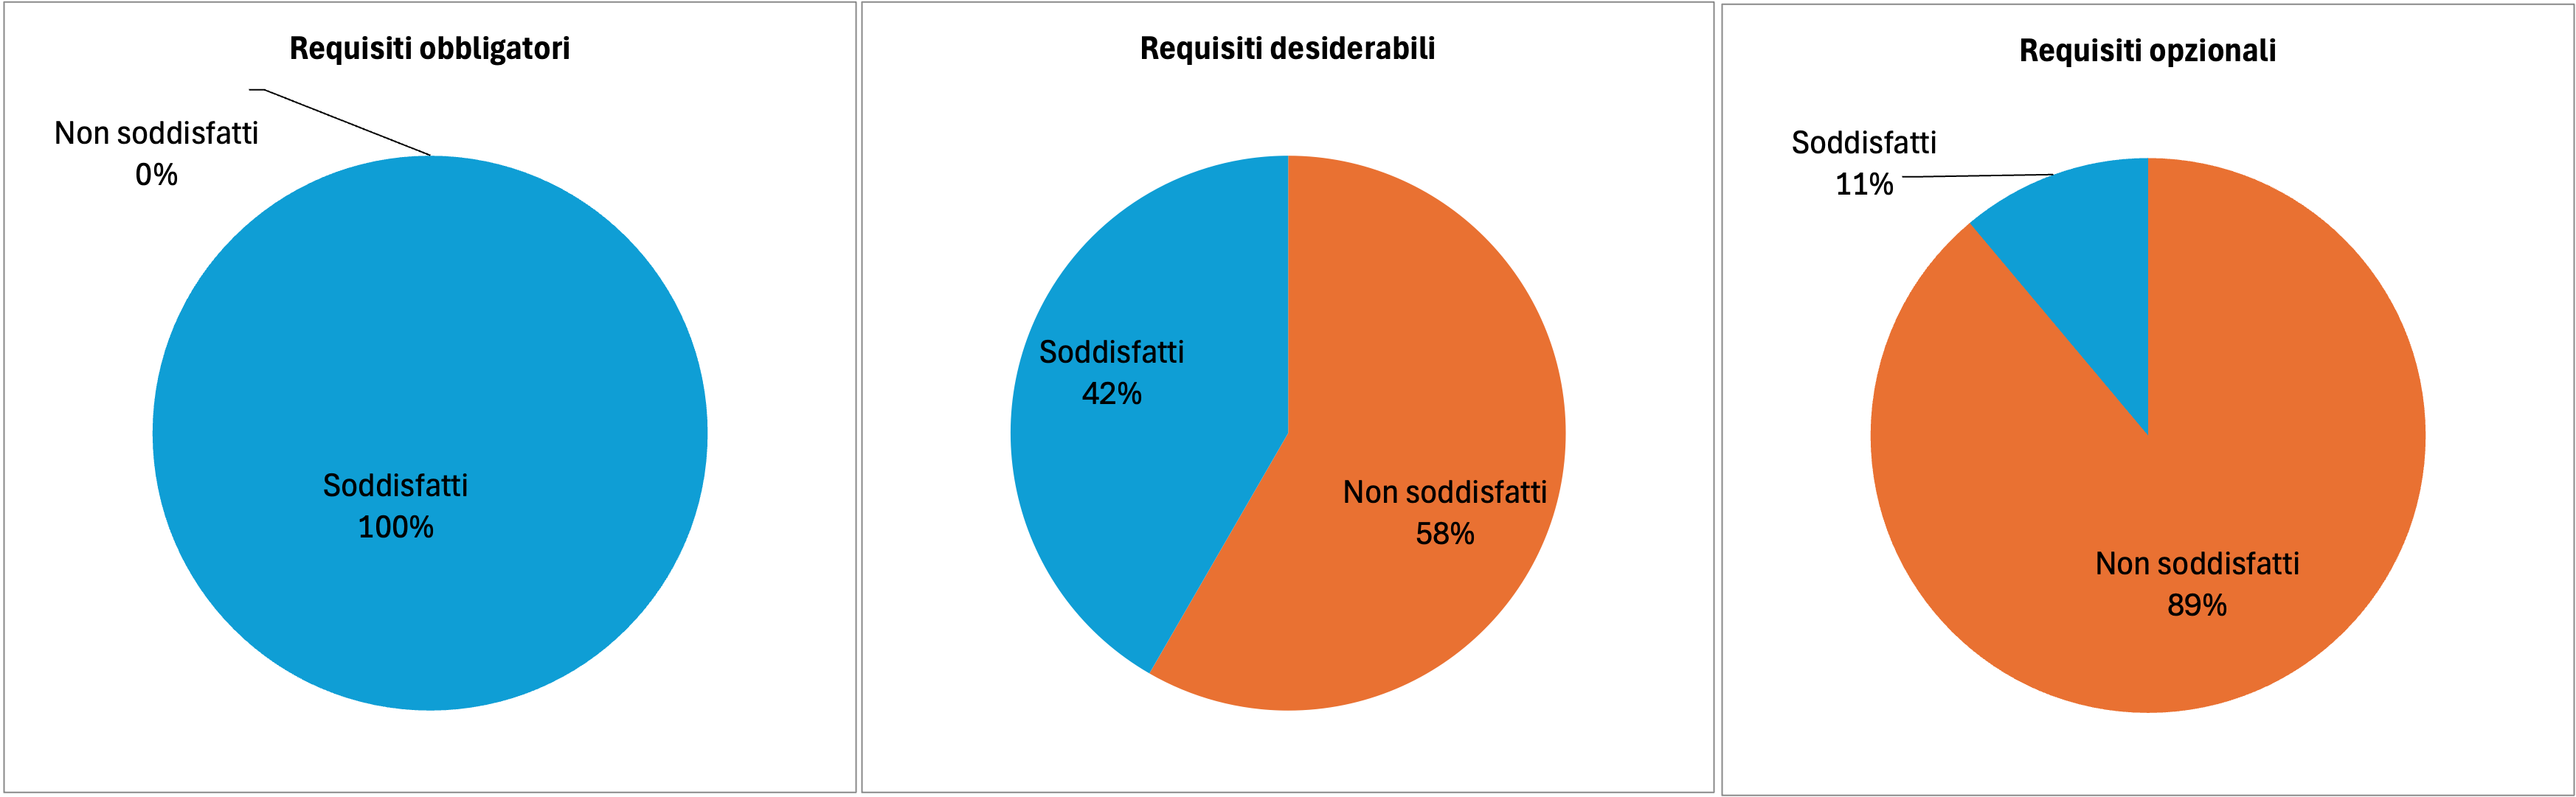
\includegraphics[width=0.8\textwidth]{./images/REQ.png}
    \caption{Requisiti soddisfatti}
\end{figure}
\subsubsubsection*{Analisi}
La copertura dei requisiti obbligatori\textsubscript{G} è del 100\%, a conferma del pieno rispetto dei criteri minimi di accettazione e dei vincoli progettuali.
I requisiti desiderabili\textsubscript{G} risultano soddisfatti al 42\%, indicando un buon livello di implementazione oltre la soglia minima, con margini di miglioramento per potenziare ulteriormente il valore del prodotto.
I requisiti opzionali\textsubscript{G} hanno una copertura del 11\%, coerente con la loro natura non prioritaria; rappresentano possibili spunti per evoluzioni future.

\subsection{Qualità di prodotto - Affidabilità}
\subsubsection{PTCP, CC}
\begin{figure}[H]
    \centering
    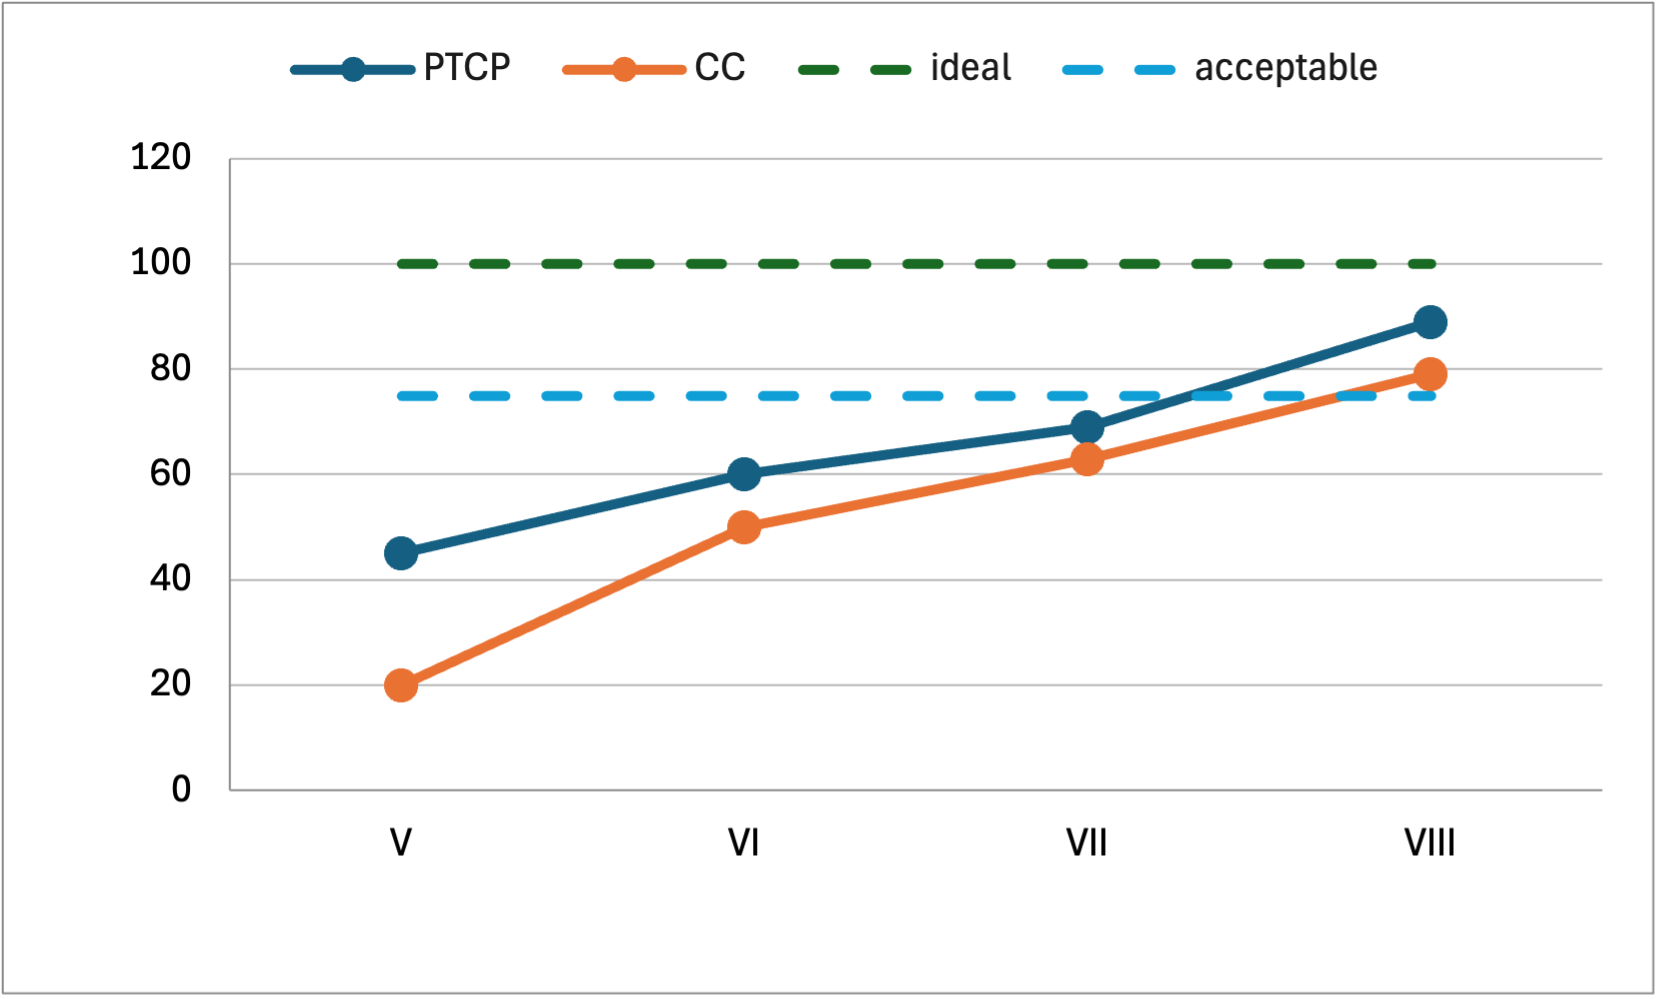
\includegraphics[width=0.8\textwidth]{./images/PTCP-CC.png}
    \caption{Passed Test Cases Percentage, Code Coverage}
\end{figure}
\subsubsubsection*{Analisi}
Nei primi periodi di lavoro sull'MVP, ci sono stati molti test falliti (probabile fase di sviluppo iniziale), ma il miglioramento in seguito dimostra un’ottima gestione dei bug e la crescita della stabilità del codice. Anche la copertura è migliorata notevolmente, questo suggerisce che, a partire dal periodo VI, si è iniziato a testare in modo più sistematico, coprendo le feature principali.